\cleardoublepage
\chapterimage{bg/10}

\chapter{Étude de genre}\label{cha:genre}



	\section{Présentation du contexte}
		Les femmes sont depuis toujours sous-représentés dans le domaine informatique, cependant au fur et à mesure de l'évolution de la société, ces disparités s'amenuisent.
		
		 Cette étude avait pour but d'étudier le statut actuel des chercheuses dans le milieu informatique par des méthodes scientométriques en se concentrant sur les membres de comités de rédaction de 77 revues scientifiques du domaine IS.
		 
		Les résultats du stage alimenteront la discussion en cours sur la représentation des femmes dans les sciences.

	
	\section{Récupération et mise en forme des données}
		Les données sur lesquelles nous devions travailler étaient celles de DBLP. Or la base contenant ces données datait de 2010 -- ayant été créée dans le cadre des précédentes recherches de Guillaume Cabanac -- et n'avait pas été mise à jour depuis. Il a donc été décidé que le plus simple était que je crée une nouvelle base contenant les données à jour, et ayant la même architecture que l'ancienne (voir figure~\ref{fig:mcdDblp}).
		
		\begin{figure}[h]
			\centering
			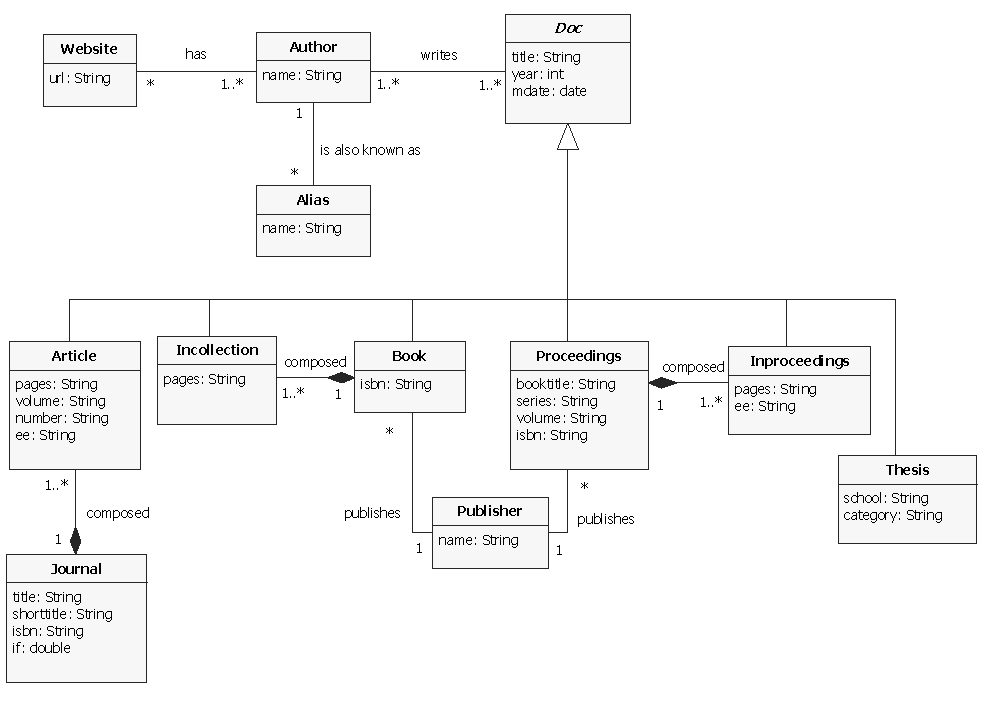
\includegraphics[width=\textwidth]{ch5/genre/dblp}
			\caption{Structure de la base de données contenant les données de DBLP}\label{fig:mcdDblp}
		\end{figure}
		
		Pour cela il a tout d'abord fallu que je récupère le fichier XML de ces données et que je le traite avec l'analyseur Java conçu par Anaïs Lefeuvre. Toute la procédure d'insertion était claire et documentée, ce qui m'a permis de savoir exactement comment procéder.
		
		 Ainsi après avoir créé les tables nécessaires et inséré les données à l'aide de Sql*Loader j'ai réactivé les indexes et les contraintes (désactivés par SQL*Loader pour des raisons de performance lors de l'insertion des données). J'ai finalement inséré les comités de rédaction des différents journaux et mis à jour le sexe et pays de chaque chercheur appartenant à un comité de rédaction grâce aux annotations manuelles réalisées par Guilaume~Cabanac.
	
		
	\section{Présentation des données et des tests utilisés}
		
		\subsection{Présentation générale des données}
			DBLP regroupe une quantité importante de données (voir tableau~\ref{tab:general}), mais notre étude s'est concentrée sur les membres de comités de rédaction de 77 journaux scientifiques du domaine IS.
			
			Les journaux dont nous connaissions les comités de rédaction sont présentés dans le tableau~\ref{tab:journaux} et les effectifs sur lesquels nous avons travaillé dans le tableau~\ref{tab:membres}.
		
			\begin{table}[h]
				\centering
				\caption{Nombre d'éléments référencés dans notre base de données.}\label{tab:general}
				\input{tableaux/ch5/genre/effGeneral}
			\end{table}
		
			\begin{table}[p]
				\centering
				\caption{Journaux du domaine IS pour lesquels nous disposions du comité de rédaction.}\label{tab:journaux}
				\input{tableaux/ch5/genre/journaux}
			\end{table}
		
			\begin{table}[h]
				\centering
				\caption{Nombre de membres de comités de rédaction référencés dans notre base de données.}\label{tab:membres}
				\input{tableaux/ch5/genre/effMembres}
			\end{table}
			
			Bien évidemment le domaine SI n'est pas représenté uniquement par ces journaux, nous ne disposions ici que d'une petite partie des membres de comités de rédaction du domaine. Étant donné le nombre de chercheurs présents dans notre base (voir tableau~\ref{tab:general}), même en prenant en compte le fait que de nombreux chercheurs ne dépendent pas du domaine SI, nous pouvions considérer qu'il s'agissait d'un échantillon d'individus indépendants et identiquement distribués.
			
			C'est la raison pour laquelle nous avons jugé pertinent de réaliser des tests statistiques afin d'inférer le comportement de la population totale des membres de comités de rédaction du domaine SI, et éventuellement suggérer, de façon très prudente, quelques tendances dans la population globale des chercheurs en SI -- les membres de comités de rédaction étant des chercheurs choisis par leurs pairs pour leur influence dans le milieu, et non séléctionnés au hasard, il est en effet difficile de savoir si leur comportement peut être généralisé au reste de la communauté.
			
	
		\subsection{Présentation des tests statistiques}
			\subsubsection{Shapiro-Wilk}
				Ce test a pour hypothèse nulle que l'échantillon testé est issu d'une population normalement distribuée et la statistique de test utilisée est
			\[
			W = \frac{\left(\sum_{i=1}^{n}a_ix_{(i)}\right)^2}{\sum_{i=1}^{n}\left(x_i-\bar{x}\right)^2}
			\]
			où
			\begin{itemize}
				\item $x_{(i)}$ désigne la ième statistique d'ordre , i.e., le ième plus petit nombre dans l'échantillon,
				\item $\bar{x}$ est la moyenne de l'échantillon,
				\item la constante $a_i$ est donnée par
					\[ (a_1, …, a_n) = \frac{m^TV^{-1}}{\sqrt{m^TV^{-1}V^{-1}m}} \]
					où $m = (m_1, …, m_n)^T$ et $m_1, …, m_n$ sont les espérances des statistiques d'ordre d'un échantillon de variables indépendantes et identiquement distribuée suivant une loi normale, et $V$ est la matrice de variance-covariance de ces statistiques d'ordre.
			\end{itemize}
			
			
			\subsubsection{Kolmogorov-Smirnov}
				Le test de Kolmogorov-Smirnov est utilisé pour déterminer si un échantillon suit bien une loi donnée connue ou bien si deux échantillons suivent la même loi. Sa statistique  vaut
			\[ D = \max\left(|F(x) - F(y)|\right)\]
			où
			\begin{itemize}
				\item $F(x)$ est la fonction de répartition du premier échantillon $(x_1, …, x_p)$,
				\item $F(y)$ est la fonction de répartition du second échantillon $(y_1, …, y_q)$.
			\end{itemize}
			
			
			\subsubsection{Wilcoxon / Mann-Whitney U}
				Le test de Wilcoxon -- aussi appelé test \emph{U} de Mann-Whitney -- permet de tester si deux échantillons ont la même loi. Sa statistique de test est
			\[ W = \sum_{i=1}^pR_i \]
			où $R_i$ est le rang de $x_i$ dans l'ensemble des $(x_1, …, x_p)$ et des $(y_1, …, y_q)$ classés par ordre croissant.

	
	\section{Répartition géographique}
		Une des premières questions auxquelles j'ai souhaité répondre a été la répartition géographique des membres féminins de comités de rédaction. Les membres de comités de rédaction étaient affiliés à 55 pays, dont 32 comptaient des membres féminins.
		
		Pour permettre une visualisation rapide des principaux pays, j’ai décidé de réaliser un histogramme avec Gnuplot, visible en figure~\ref{fig:pays} -- pour des raisons de place seuls les  20 pays ayant au moins trois membres féminins de comités de rédaction sont visibles.
			
		\begin{figure}[p]
			\centering
			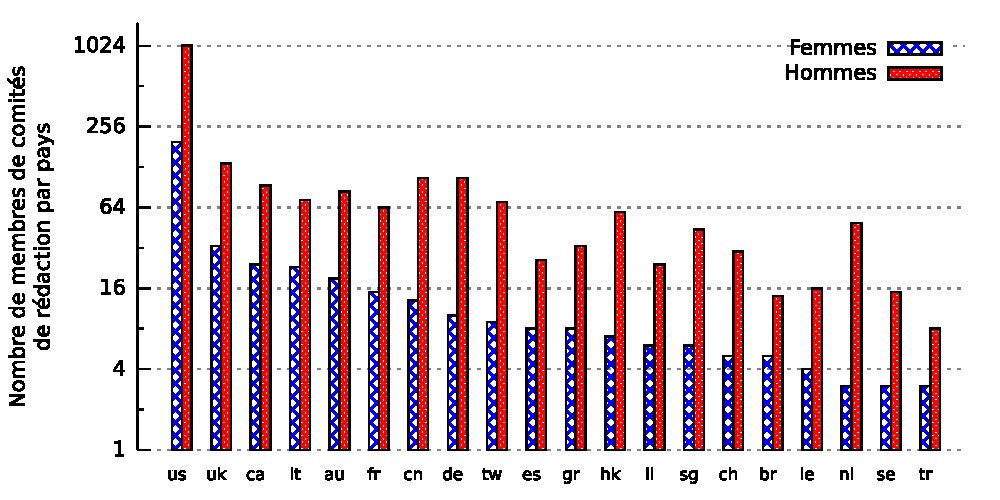
\includegraphics[width=\textwidth]{ch5/genre/pays}
			\caption{Pays des membres féminins de comités de rédaction -- à titre de
comparaison le nombre de membres masculins de chaque pays est également indiqué -- pour des raisons de place seuls les 20 pays ayant au moins trois membres féminins apparaissent ici.}\label{fig:pays}
		\end{figure}
			
		Pour mieux visualiser la différence entre le nombre de membres masculins et féminins j’ai décidé de réaliser un autre histogramme avec cette fois-ci la proportion de membres féminins pour chacun des pays figurant dans l’histogramme précédant.
			
		\begin{figure}[p]
			\centering
			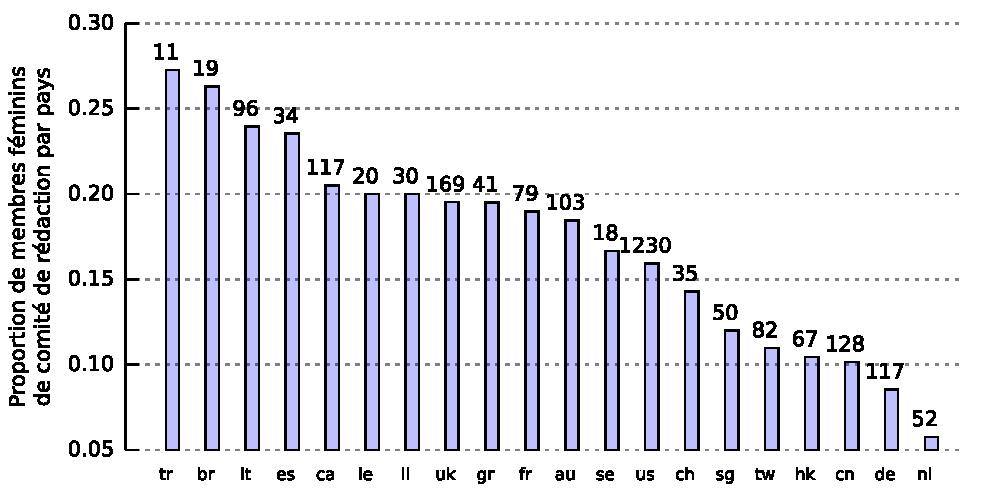
\includegraphics[width=\textwidth]{ch5/genre/paysProp}
			\caption{Proportion des membres féminins de comités de rédaction des 20
pays figurant dans la figure~\ref{fig:pays} -- le nombre total de membres de comités de rédaction du pays est indiqué au dessus de la colonne correspondante.}\label{fig:paysProp}
		\end{figure}
		
		On constate que le pays le plus paritaire \footnote{Se dit d’une assemblée formée de représentants en nombre égal des parties en présence -- dans notre cas une assemblée comptant autant d’hommes que de femmes.} est la Turquie, bien que les femmes ne représentent qu’environ 27\% des membres de comités de rédaction -- il faut cependant noter que la Turquie ne possède que 11 membres de comités de rédaction.
			
		Ces premières analyses confirment nos impressions initiales sur la sous-représentation des femmes dans le domaine SI. En effet dans notre cas seul 58\% des pays comprennent des membres féminins de comités de rédaction et ces membres n'atteignent jamais le tiers de membres totaux de leur pays. On peut également noter que même les pays ayant politique de recherche très favorable, tels que les États-Unis, ne sont pas épargnés par cette sous-représentation.


	\section{Comparaison de générations}
		En me documentant sur les différentes études de genre déjà réalisées j'ai pris connaissance de l'article \citep*{van} comparant la différence de productivité entre hommes et femmes entre deux générations de chercheurs.
		
		\citet*{van} constatent dans cet article que cette différence -- clairement établie dans la génération de chercheurs établis pour laquelle les hommes produisent plus que les femmes -- a tendance a disparaître voire à s'inverser dans le domaine des sciences sociales. J'ai pensé qu'il pourrait être intéressant d'analyser nos données de la même façon afin de voir s'il y avait une évolution, positive ou négative, de la place des femmes dans la communauté SI.
	
		Afin de déterminer les limites des générations de chercheurs à comparer j'ai choisi de me baser sur la date du premier document -- article publié, livre ou participation à une conférence -- archivé sur DBLP.
		
		À partir de ces dates j'ai divisé les chercheurs comme suit~:
		\begin{itemize}
			\item une «~ancienne~» génération de chercheurs ayant réalisé leur premier document avant 2000,
			\item une «~nouvelle~» génération de chercheurs ayant réalisé leur premier document après ou en 2000.
		\end{itemize}
		
		L'année 2000 a été choisie comme limite car les articles lus suggéraient que l'écart de production observé entre hommes et femmes se creusait principalement durant les dix premières années de carrières, il fallait donc que ma nouvelle génération commence au plus tard en 2003. Afin d'avoir une quantité suffisamment importante de données à analyser j'ai décidé de la faire commencer un peu plus tôt, et donc de sélectionner une date facilement repérable, comme 2000.
		
		Les \numprint{2850} membres de comités de rédaction étaient donc répartis selon les effectifs présentés dans le tableau~\ref{tab:eff} -- le total ne vaut pas \numprint{2850} car je n'ai pris en compte que les chercheurs pour lesquels le sexe était clairement déterminé.
		
		\begin{table}[ht]
			\centering
			\caption{Répartition des membres de comités de rédaction -- les 26 chercheurs pour lesquels le genre n'a pas pu être déterminé ne sont pas pris en compte ici.}\label{tab:eff}
			\input{tableaux/ch5/genre/effGen}
		\end{table}
		
		
		\subsubsection{Production et productivité}			
			Le premier élément que j'ai souhaité tester a été la production des chercheurs. En effet il a souvent été noté une différence significative d'articles produits entre hommes et femmes \citep*{Nakhaie2002, Prpic2002, PenasWillett2006, bramoAngeloCaprasecca2009, BraisherGorringeElgar2006, BornmannGannonWallon2007, washburn2006, 1998}. Je souhaitais donc voir si cette différence avait tendance à disparaître avec les années.
			
			Pour calculer la production d'un chercheur j'ai décidé d'utiliser la métrique de production présentée dans \citep*{geometric} ayant pour formule~:
		\[g(r,n) = \frac{2^{n-r}}{2^n-1}\]
		avec $n \in \mathbb{N}^*_+$ le nombre total d'auteurs du document et $r \in \mathbb{N}^*_+$ le rang du chercheur dans la liste de ceux-ci.
			
			Les productions selon le genre de l'ancienne et de la nouvelle génération ainsi calculées sont représentées en figures~\ref{fig:prod-g1} et \ref{fig:prod-g2}.
			
			\begin{figure}[p]
				\centering
				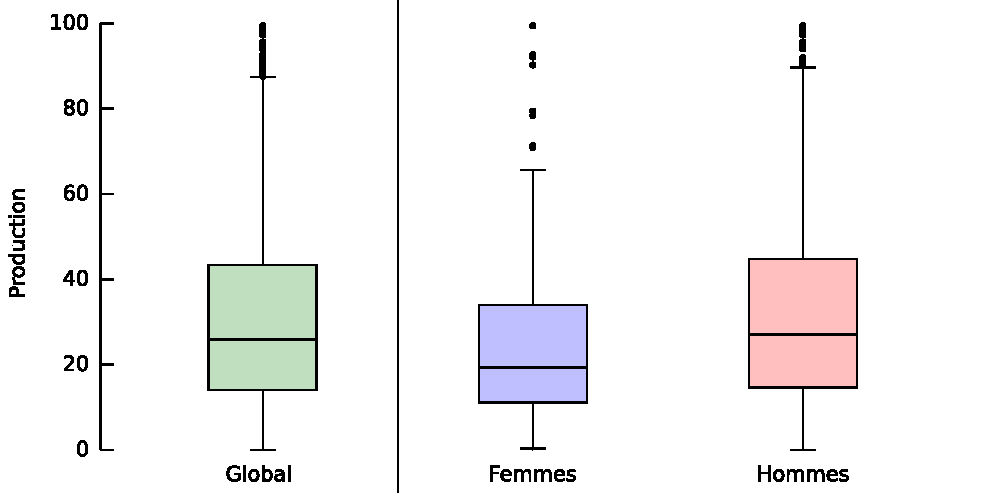
\includegraphics[width=\textwidth]{ch5/genre/prod-g1}
				\caption{Production de l'ancienne génération de chercheurs par genre -- les
78 chercheurs (3,5\% de la génération) ayant une production supérieure à 100 n’apparaissent pas sur ce graphique.}\label{fig:prod-g1}
			\end{figure}
			
			\begin{figure}[p]
				\centering
				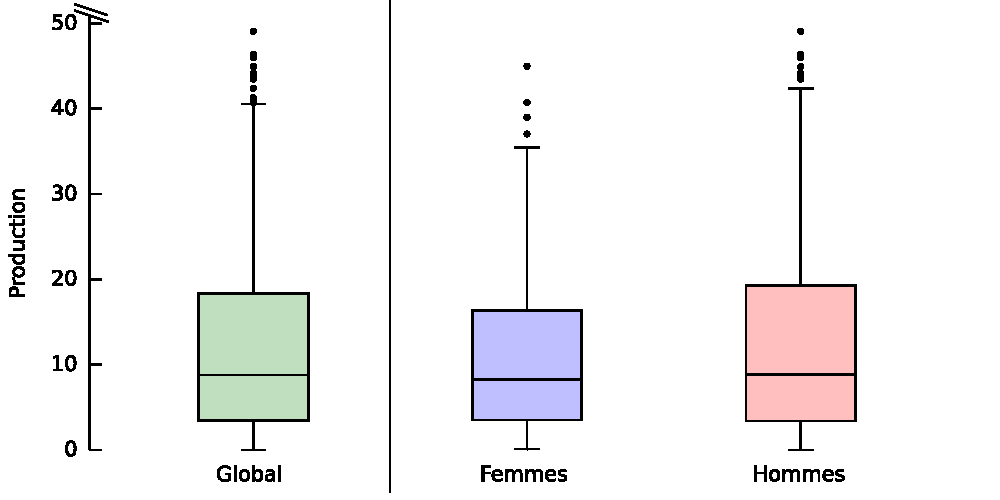
\includegraphics[width=\textwidth]{ch5/genre/prod-g2}
				\caption{Production de la nouvelle génération de chercheurs par genre -- les
20 chercheurs (3,5\% de la génération) ayant une production supérieure à 50 n’apparaissent pas sur ce graphique.}\label{fig:prod-g2}
			\end{figure}
			
			On constate que la différence clairement visible pour l'ancienne génération (où la médiane pour les femmes vaut 19,38 et celle des hommes 27,13, soit un delta de 7,75) s'atténue fortement pour la nouvelle (où cette fois-ci la médiane pour les femmes vaut 8,24 contre 8,84 pour les hommes, soit un delta de 0,60).
			
			Afin d'en avoir le c\oe ur net j'ai décidé d'effectuer des tests statistiques pour déterminer~:
			\begin{enumerate}
				\item si la différence de production entre hommes et femmes était significative,
				\item si cette différence diminuait avec le temps.
			\end{enumerate}
			
			Afin de choisir quels tests utiliser pour cela, j'ai tout d'abord choisi de vérifier la normalité de mes échantillons représentant la productivité des chercheurs et chercheuses de chaque génération avec un test de Shapiro-Wilk. Les résultats de ces tests sont présentés dans le tableau~\ref{tab:testsNorm}. On peut voir qu'aucun de mes échantillons n'est distribué selon la loi normale -- les \textit{p-values} étant largement inférieures à 5\%.
			
			\begin{table}[ht]
				\centering
				\caption{Résultats du test de Shapiro-Wilk sur les échantillons «Production des chercheuses de l'ancienne génération», «Production des chercheurs de l'ancienne génération», «Production des chercheuses de la nouvelle génération» et «Production des chercheurs de la nouvelle génération», indiquant si ces échantillons suivent une loi normale.}\label{tab:testsNorm}
				\input{tableaux/ch5/genre/prodTestNorm}
			\end{table}
			
			Étant donné que nous ne connaissont pas la loi de ceux-ci, j'ai décidé d'utiliser des tests non paramétriques -- Kolmogorov-Smirnov et Wilcoxon -- pour les comparer. Les résultats de ces tests sont visibles dans le tableau~\ref{tab:tCompProd}. On peut voir que les deux nous permettent de tirer les même conclusions :
			\begin{itemize}
				\item la différence de production entre membres masculins et féminins des comités de rédaction de l'ancienne génération est significative d'un point de vue statistique,
				\item cette différence s'est atténuée au point de ne plus être significative pour la nouvelle génération.
			\end{itemize}
			
			\begin{table}[p]
				\centering
				\caption{Résultats des tests de Kolmogorov-Smirnov (KS) et Wilcoxon (W) indiquant si la différence de production entre hommes et femmes est significative.}\label{tab:tCompProd}
				\input{tableaux/ch5/genre/prodTestGen}
			\end{table}
			
			
			Cette démarche présentait néanmoins un biais non négligeable : au sein d’une même génération, deux chercheurs peuvent avoir une durée de carrière très dissemblable. Pour pallier ce problème j’ai décidé, sur une suggestion de Guillaume, de diviser la production
de chaque chercheur par la durée de sa carrière (calculée en fonction du plus ancien et du plus récent de ses document présents dans la base) afin d'obtenir sa productivité annuelle. J’ai également écarté les membres ayant participé à la rédaction de moins de 5 documents, ce qui nous donne de nouveaux effectifs, présentés dans le tableau~\ref{tab:effNew}. Nous obtenons donc la productivité annuelle par chercheur visible dans les figures~\ref{fig:prodAng1} et \ref{fig:prodAng2}.
		
		\begin{table}[h]
			\centering
			\caption{Répartition des membres de comités de rédaction -- les chercheurs pour lesquels le genre n\rq{}a pas pu être déterminé et ceux ayant participés à la rédaction de moins de 5 documents ne sont pas pris en compte ici.}\label{tab:effNew}
			\begin{tabular}{l >{\raggedleft}m{0.15\textwidth}<{\raggedleft} >{\raggedleft}m{0.15\textwidth} m{0.15\textwidth}<{\raggedleft}}
				\toprule
				& Femmes		& Hommes	& Total			\\
				\midrule
				Ancienne génération	& 284	& 1849	& 2171	\\
				Nouvelle génération	& 116	& 446	& 562	\\ 
				\midrule
				Total					& 400	& 2295	& 2695	\\
				\bottomrule
			\end{tabular}
		\end{table}
			
			\begin{figure}[p]
				\centering
				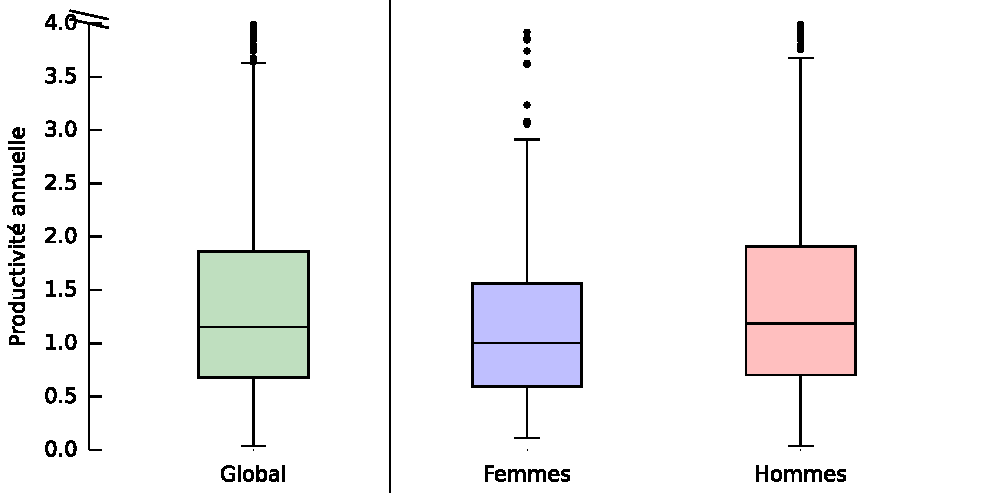
\includegraphics[width=\textwidth]{ch5/genre/prodAng1}
				\caption{Productivité annuelle de l\rq{}ancienne génération de chercheurs par genre -- les 74 chercheurs (3,5\% de la génération) ayant une productivité annuelle supérieure à 4 n'apparaissent pas sur ce graphique.}\label{fig:prodAng1}
			\end{figure}
			
			\begin{figure}[p]
				\centering
				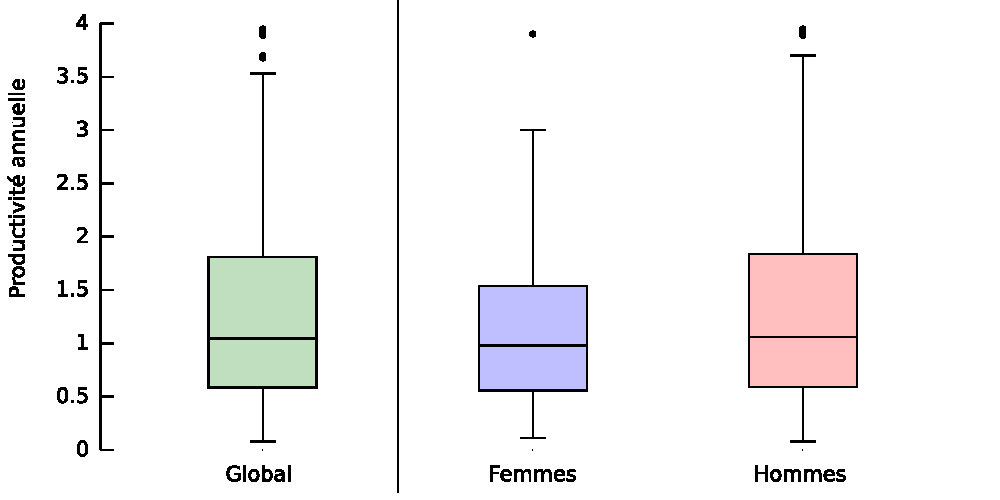
\includegraphics[width=\textwidth]{ch5/genre/prodAng2}
				\caption{Productivité annuelle de l\rq{}ancienne génération de chercheurs par genre -- les 74 chercheurs (3,5\% de la génération) ayant une productivité annuelle supérieure à 4 n'apparaissent pas sur ce graphique.}\label{fig:prodAng2}
			\end{figure}
			
			Là encore on observe une différence plus importante entre hommes et femmes pour l'ancienne génération (1,00 pour les femmes contre 1,19 pour les hommes) que pour la nouvelle (où la médiane des femmes vaut 0,98 contre 1,06 pour les hommes).
			
			J'ai suivi la même démarche que pour les résultats précédents, les résultats du test de Shapiro-Wilk est visible dans le tableau~\ref{tab:testsNormBis}. On peut voir qu'ici encore aucun de mes échantillons n'est distribué selon la loi normale -- les \textit{p-values} étant largement inférieures à 5\%. J'ai donc réutilisé les même tests que précédemment, les résultats sont visibles dans le tableau~\ref{tab:tCompProdBis}.
			
			\begin{table}[ht]
				\centering
				\caption{Résultats du test de Shapiro-Wilk sur les échantillons «Productivité annuelle des chercheuses de l'ancienne génération», «Productivité annuelle des chercheurs de l'ancienne génération», «Productivité annuelle des chercheuses de la nouvelle génération» et «Productivité annuelle des chercheurs de la nouvelle génération», indiquant si ces échantillons suivent une loi normale.}\label{tab:testsNormBis}
				\input{tableaux/ch5/genre/prodTestNormBis}
			\end{table}
			
			\begin{table}[hb]
				\centering
				\caption{Résultats des tests de Kolmogorov-Smirnov (KS) et Wilcoxon (W) indiquant si la différence de productivité annuelle entre hommes et femmes est significative.}\label{tab:tCompProdBis}
				\input{tableaux/ch5/genre/prodTestGenBis}
			\end{table}
			
			Ces nouvelles analyses nous donnent donc le même résultat que les précédentes~: l'écart de production entre hommes et femmes tend à diminuer voire à disparaître avec le temps.
		
		
		\subsubsection{$\varphi$-index}
			J'ai ensuite pensé qu'il serait intéressant de comparer également l'évolution du $\varphi$-index entre générations. Le $\varphi$-index mesure la \textit{partnership ability} -- l'aptitude à collaborer avec d'autres chercheurs et à conserver des collaborations. J'ai calculé cette mesure à l'aide de l'article \citep{partnership}. Les boîtes à moustaches correspondantes sont visibles en figures~\ref{fig:phi-g1} et \ref{fig:phi-g2}.
			
			\begin{figure}[p]
				\centering
				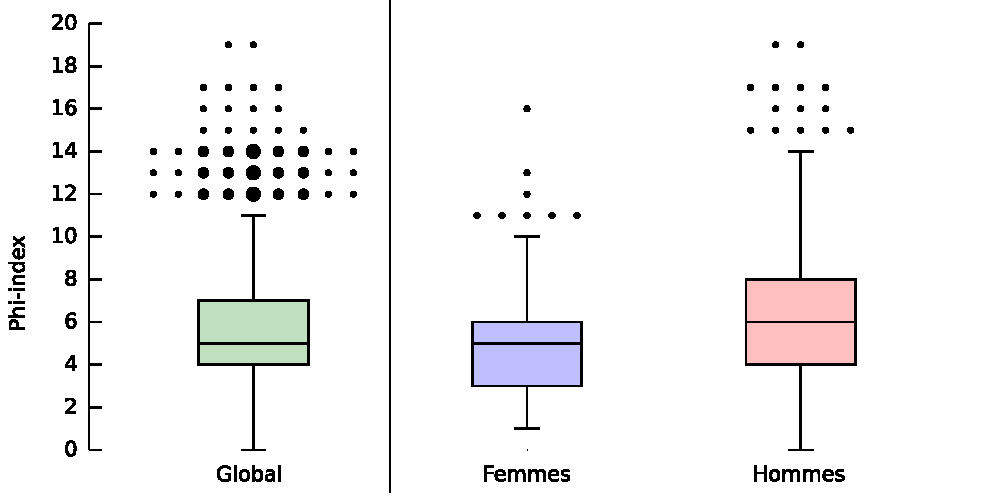
\includegraphics[width=\textwidth]{ch5/genre/phi-g1}
				\caption{$\varphi$-index de l'ancienne génération de chercheurs par genre}\label{fig:phi-g1}
			\end{figure}
			
			\begin{figure}[p]
				\centering
				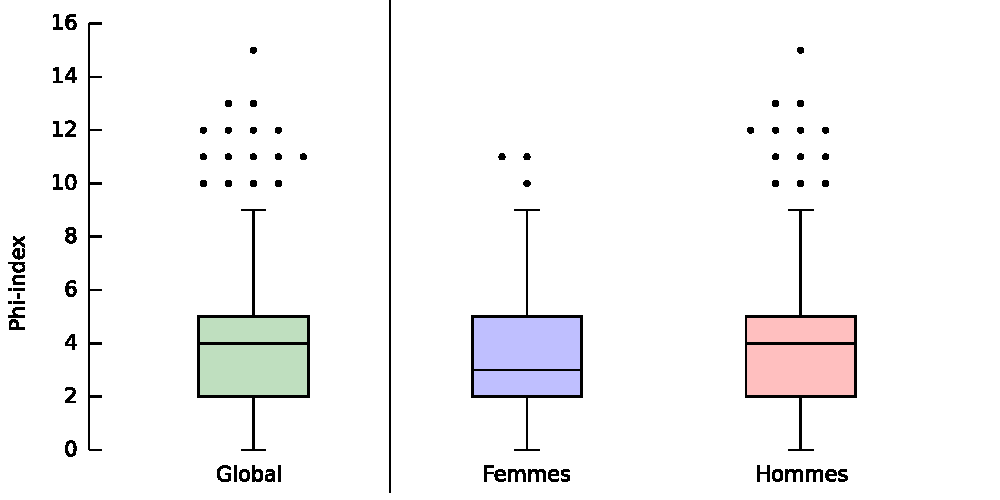
\includegraphics[width=\textwidth]{ch5/genre/phi-g2}
				\caption{$\varphi$-index de la nouvelle génération de chercheurs par genre}\label{fig:phi-g2}
			\end{figure}
			
			On peut voir que même si la médiane du $\varphi$-index est légèrement inférieure à celle des hommes dans la nouvelle génération, la différence est tout de même beaucoup moins flagrante que pour l'ancienne génération.
			
			J'ai décidé d'appliquer la même démarche statistique que pour la production étant donné qu'ici aussi mes échantillons ne suivaient pas une loi normale (voir tableau~\ref{tab:testsNormPhi}.
			
			\begin{table}[ht]
				\centering
				\caption{Résultats du test de Shapiro-Wilk sur les échantillons «$\varphi$-index des chercheuses de l'ancienne génération», «$\varphi$-index des chercheurs de l'ancienne génération», «$\varphi$-index des chercheuses de la nouvelle génération» et «$\varphi$-index des chercheurs de la nouvelle génération», indiquant si ces échantillons suivent une loi normale.}\label{tab:testsNormPhi}
				\input{tableaux/ch5/genre/phiTestNorm}
			\end{table}
			
			\begin{table}[p]
				\centering
				\caption{Résultats des tests de Kolmogorov-Smirnov (KS) et Wilcoxon (W) indiquant si la différence de $\varphi$-index entre hommes et femmes est significative.}\label{tab:tCompPhi}
				\input{tableaux/ch5/genre/phiTestGen}
			\end{table}
			
			On constate que, comme pour la productivité, les deux tests nous donnent les même résultats (voir tableau~\ref{tab:tCompPhi})~:
			\begin{itemize}
				\item la différence de $\varphi$-index entre membres masculins et féminins des comités de rédaction de l'ancienne génération est significative,
				\item cette différence s'est atténuée au point de ne plus être significative pour la nouvelle génération.
			\end{itemize}
	

	\section{Conclusions de l'étude}
		Toutes les analyses menées sur les membres de comités de rédaction de des 77 principales revues du domaine SI nous permettent de tirer plusieurs conclusions.
		
		Tout d'abord la sous-représentation majeure des femmes est un problème global : des 55 pays auxquels sont affiliées les membres féminins de comités de rédaction, seuls 32 comprennent des membres féminins, soit seulement 58\%. Parmi ces 32 pays seuls deux ont plus de 30\% de membres féminins : la Croatie qui a deux membres féminins et la Slovénie qui a 2 membres féminins et 4 membres masculins.
		
		Nous pouvons ensuite noter que l'écart de productivité et de $\varphi$-index entre hommes et femmes observé dans de nombreux papiers scientifiques -- et pouvant constituer une «~justification~» de la quasi absence des femmes aux postes de pouvoir, celles-ci étant supposément moins performante que les hommes -- tend à diminuer voire à disparaître dans les nouvelles générations de chercheurs.
		
		
	
